\chapter{Resultados}

Neste capítulo são apresentados os resultados obtidos nos testes de carga e busca dos dados. Os testes foram realizados em três configurações de \emph{cluster}, com duas, quatro e seis máquinas, a fim de se analisar a melhora do desempenho de um banco de dados não relacional ao se aumentar o número de nós. Além disso, em cada configuração de \emph{cluster}, foram realizados testes com dois volumes distintos de dados.

Em cada configuração de teste foram realizadas dez repetições, tanto na inserção quanto na busca, a fim de garantir resultados mais consistentes. 

\section{Carga de dados}
A carga de dados foi realizada a partir da leitura dos arquivos \emph{.csv} de dados do Bolsa Família, com seleção das colunas a serem utilizadas e tratamento de alguns campos.
Os dados foram carregados a partir de uma única máquina utilizando aplicação desenvolvida, sendo o \emph{Cassandra} responsável pela distribuição dos mesmos dentro do \emph{cluster} . Foi feita também uma comparação entre os tempos observados em cada uma das configurações utilizadas. Esta seção descreve em detalhes essas operações.

\subsection{Preparação e carga}
Foi desenvolvida uma aplicação Java responsável por toda a operação da inserção dos dados com uso do \emph{driver} da \emph{Datastax}. A aplicação realiza a leitura dos dados à partir dos arquivos .csv e utiliza apenas os campos que serão utilizados na família de colunas do banco de dados: \textbf{UF, Código SIAFI Município, Nome Município, NIS Favorecido, Nome Favorecido, Fonte-Finalidade, Valor Parcela, Mês Competência}. 

Para a correta inserção no banco Cassandra alguns campos tiveram seus valores tratados pela aplicação. No campo Valor Parcela foi necessária a remoção do separador de milhares(',') para se adequar ao tipo \emph{double} do Cassandra. Para o campo Mês Competência, que originalmente segue o padrão MM/AAAA, não é suportado pelo Cassandra, foi necessária a inclusão de um dia para a correta utilização do tipo \emph{timestamp}, sendo então armazenado no formato DD/MM/AAAA.

A carga foi realizada com dois volumes de dados, correspondentes a um dezoito meses, e trinta meses de informações do Bolsa Família, a fim de se analisar o desempenho do banco com diferentes números de nós ao se aumentar o volume de dados. A Tabela~\ref{tab:volume} apresenta o tamanho total dos dados inseridos em cada uma dessas cargas.

\begin{table}[]
	\centering
	\caption{Volume da dados}
	\label{tab:volume}
	\begin{tabular}{ll}
		\textbf{Carga} & \textbf{Tamanho} \\ \hline
		18 meses     &  8,79 GB              \\ \hline
		30 meses    &  14,69 GB             \\ \hline
	\end{tabular}
\end{table}

A inserção foi realizada de maneira assíncrona com uso de funções disponibilizadas pelo \emph{driver} da \emph{Datastax}. A \emph{query} em formato CQL~\ref{lst:cql_insert} é montada e tem seus parâmetros substituidos, e então ela é executada com o comando \emph{executeAsync} da classe \emph{Session} do \emph{driver}. São realizadas operações em seis \emph{threads} simultâneas, valor que apresentou o melhor resultado nos testes realizados.

Os testes foram realizados para as configurações de \emph{cluster} com duas, quatro e seis máquinas, com objetivo de analisar uma possível melhora no desempenho em \emph{clusters} maiores.

\begin{lstlisting}[caption={Código CQL para inserção},label={lst:cql_insert},language=SQL]
INSERT INTO bolsa_familia.dados (uf, cod_municipio, nome_municipio, nis_favorecido, nome_favorecido, fonte, valor, periodo) VALUES (?, ?, ?, ?, ?, ?, ?, ?)
\end{lstlisting}

A Tabela~\ref{tb_insert} apresenta os tempos obtidos na inserção dos dados nos diferentes ambientes e volumes de dados. O gráfico~\ref{fig:graph_insert} apresenta os mesmo dados para melhor visualização.


\begin{table}[]
	\centering
	\caption{Inserção}
	\label{tb_insert}
	\begin{tabular}{lllll}
		\textbf{Tamanho}	& \textbf{2 nós} & \textbf{4 nós} & \textbf{6 nós} \\ \hline
		\textbf{18 meses}   	& 1h         	 & 55m       	  & 52m            \\ \hline
		\textbf{30 meses}     & 2h31m      	 & 2h19m          & 2h06m          \\ \hline
	\end{tabular}
\end{table}

Com o aumento do número de máquinas, foi observada uma melhora média de \emph{6,46\%} quando utilizado o volume de carga correspondente a 18 meses, e {8,54\%} nos dados de 30 meses, como exposto na tabela~\cite{tb:comparativo_insert}. Esse resultado demonstra a utilidade do Cassandra ao se trabalhar com um crescente volume de dados.

\begin{table}[]
	\centering
	\caption{Comparativo dos tempos de Inserção}
	\label{tb:comparativo_insert}
	\begin{tabular}{|l|c|c|l}
		\cline{1-3}
		\textbf{2 para 4 máquinas} & \textbf{4 para 6 máquinas} & \textbf{Média}  &  \\ \cline{1-3}
		8,70\%                     & 4,22\%                     & \textbf{6,46\%} &  \\ \cline{1-3}
		8,94\%                     & 6,30\%                     & \textbf{7,62\%} &  \\ \cline{1-3}
		8,13\%                     & 8,94\%                     & \textbf{8,54\%} &  \\ \cline{1-3}
	\end{tabular}
\end{table}

\begin{figure}[!htb]
	\centering
	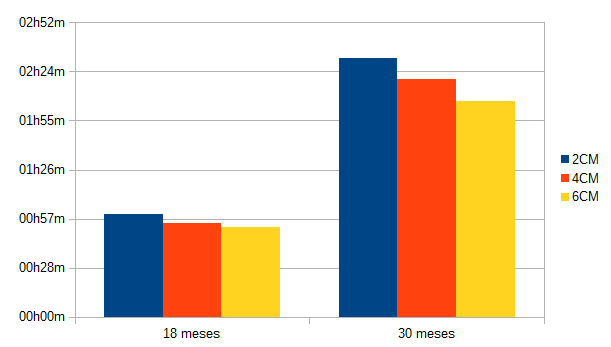
\includegraphics[width=1\textwidth]{figuras/graphinsert.png}
	\caption{Inserção de dados}
	\label{fig:graph_insert}
\end{figure}

\section{Extração de dados}
Após cada inserção dos dados, nas três configurações de \emph{cluster} (duas, quatro e seis máquinas), e com os dois volumes distintos de dados, foram realizadas consultas para verificar o desempenho de um banco de dados Cassandra ao se realizar extração de dados.

\subsection{Consultas}
Assim como para a carga de dados, foi desenvolvida uma aplicação Java para a realização das consultas no banco de dados, com uso do \emph{driver} da \emph{Datastax}. Cada teste de consulta envolveu a execução de trinta \emph{Selects} no banco, sendo que cada um realiza uma consulta com uso da linguagem CQL a um registro específico, selecionado de forma aleatória. Essa consulta, exemplificada em \ref{lst:cql_select}, contém toda a totalidade da chave primária da tabela, requisito imposto pelo banco de dados Cassandra. Cada teste foi repetido dez vezes a fim de se obter uma média dos resultados encontrados.

\begin{lstlisting}[caption={Consulta CQL},label={lst:cql_select},language=SQL]
SELECT * FROM dados WHERE nis_favorecido = 00020915229557 AND periodo = '2014-07-01' AND valor = 147.00 
\end{lstlisting}

A tabela \ref{tab:select_busca} apresenta os tempos obtidos na consulta de registros nos diferentes ambientes e volumes de dados testados. O gráfico \ref{fig:graph_select_busca} apresenta os mesmos dados para melhor visualização.

\subsection{Comparação dos ambientes}
O aumento do número de máquinas no \emph{cluster} apresentou uma melhora média de 46,20\% ao se trabalhar com dados de dezoito meses, e 66,85\% com 30 meses. Esse resultado, assim como o observado na inserção dos dados, também revela a melhoria do desempenho do Cassandra em um ambiente com um volume maior de dados.

\begin{table}[]
	\centering
	\caption{Busca de dados}
	\label{tab:select_busca}
	\begin{tabular}{lllll}
		\textbf{Tamanho} & \textbf{2 nós} & \textbf{4 nós} & \textbf{6 nós} \\ \hline
		18 meses         & 10,26 s        & 1,95 s        & 1,73 s        \\ \hline
		30 meses         & 12,98 s        & 4,38 s        & 1,43 s         \\ \hline
	\end{tabular}
\end{table}

\begin{figure}[!htb]
	\centering
	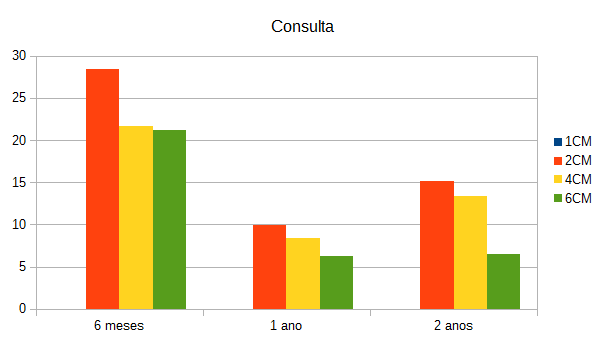
\includegraphics[width=1\textwidth]{figuras/graph_select_buscas.png}
	\caption{Busca de dados}
	\label{fig:graph_select_busca}
\end{figure}